\documentclass[11pt,a4paper]{article}

% ---------- academic paper look ----------
\usepackage[T1]{fontenc}
\usepackage[utf8]{inputenc}
\usepackage{tgtermes}
\usepackage[margin=2.5cm,top=2.4cm,bottom=2.6cm]{geometry}
\usepackage{graphicx,booktabs,xcolor,colortbl,tcolorbox,caption,enumitem,setspace,amsmath,float}
\usepackage[hidelinks]{hyperref}

\definecolor{ecink}{HTML}{1A2430}
\definecolor{ecgray}{HTML}{5A6572}
\definecolor{sigok}{HTML}{DDF2E4}
\definecolor{citeblue}{HTML}{2A5DB0}

\captionsetup{font={small},labelfont={bf},
              justification=justified,singlelinecheck=false}
\renewcommand{\topfraction}{0.85}
\renewcommand{\bottomfraction}{0.6}
\renewcommand{\textfraction}{0.15}
\renewcommand{\floatpagefraction}{0.8}
\makeatletter
\setlength{\@fptop}{0pt}
\setlength{\@fpsep}{26pt plus 6pt}
\setlength{\@fpbot}{0pt plus 1fil}
\makeatother
\setlength{\intextsep}{16pt plus 4pt minus 2pt}
\setlength{\textfloatsep}{18pt plus 4pt minus 2pt}
\setlength{\parskip}{5pt}\setlength{\parindent}{0pt}
\linespread{1.14}
\color{ecink}

\newcommand{\fignote}[1]{\par\vspace{4pt}%
  \begin{minipage}{\linewidth}\footnotesize\color{ecgray}#1\end{minipage}}

\begin{document}

% ---------- title page ----------
\begin{center}
{\fontsize{20}{26}\selectfont\bfseries
Who Leaves Teaching, and Why?\par}
\vspace{8pt}
{\fontsize{15}{20}\selectfont\bfseries
The Anatomy of Teacher Attrition in the United States, 2005--2024\par}

\vspace{26pt}
{\large \href{https://sites.google.com/view/joseeliasduranroa}{José Elías Durán Roa}\footnote{PhD Candidate in Economics,
University of Alicante, and Research Intern at the OECD Directorate for
Education and Skills. E-mail\,
\href{mailto:joseelias.duranroa@ocde.org}{joseelias.duranroa@ocde.org} and
\href{mailto:joduran@ua.es}{joduran@ua.es}. The views expressed here are
mine and do not represent those of the OECD. All remaining errors are my
own.}}

\vspace{8pt}
{\small July 2026}
\end{center}

\vspace{22pt}
\begin{center}
\begin{minipage}{0.86\textwidth}
{\fontsize{10.5}{14.5}\selectfont
\begin{center}\bfseries Abstract\end{center}\vspace{2pt}
Roughly 8 percent of American teachers leave the profession each year, a
rate that has barely moved since the early 1990s---yet almost everything
policy-relevant about that number lies in a decomposition that existing
work does not provide. Using two decades of Current Population Survey
March supplements (2005--2024), I document not just how many teachers
leave but who they are, where they go, and what the move costs them. Of
every 100 leavers, 62 exit the labor force altogether---38 at retirement
ages, 24 before 55---12 become unemployed, and only 26 hold another job a
year later, a fifth of those still inside education. Leaving is
predicted by the shape of the job, not the person: teaching part of the
year or part-time dominates every demographic trait, and pension coverage
locks teachers in. The family margin is the exception, and it is
distinctively large in teaching: a new baby raises a female teacher's
probability of leaving by 5.9 percentage points, two to three times the
effect in nursing, accounting, or law. For those who do move to another
job, leaving is a gamble rather than a raise: the median switcher gains
15 log points, but the tenth percentile loses 85, and nearly half of all
leavers report no earnings at all the following year. Measured
identically, teachers leave at the nurse benchmark, five points below
social workers, and the ordering has not changed in thirty years. An
appendix validates the retrospective instrument person-by-person against
a linked monthly panel built from the raw CPS files---the first such
audit in this literature---and a second appendix replicates Harris and
Adams (2007) on the modern decades.}
\end{minipage}
\end{center}

\clearpage
\section*{1. Introduction}

Teachers are the main school input in the production of student
achievement (\textcolor{citeblue}{Rivkin, Hanushek and Kain, 2005; Chetty,
Friedman and Rockoff, 2014}), and replacing one is costly and disruptive
for the students left behind (\textcolor{citeblue}{Ingersoll, 2001;
Ronfeldt, Loeb and Wyckoff, 2013}). Whether teachers are abandoning the
profession, and which ones, is accordingly a perennial question of
education policy---and one where the public debate runs well ahead of the
data. Announcements of a post-pandemic exodus coexist with federal
statistics showing single-digit attrition; a rich descriptive literature
reports turnover levels but stops, almost uniformly, at the schoolhouse
door, without following the leaver into her next job, her next paycheck,
or her reasons.

The data to go further have existed, in public form, for decades. The
March supplement of the Current Population Survey asks every adult two
questions that bracket a teacher's exit: the occupation of the longest
job held last calendar year, and what she is doing in the survey week.
\textcolor{citeblue}{Harris and Adams (2007)} used this instrument to
establish the level of teacher attrition for 1992--2001 and to benchmark
it against nurses, social workers, and accountants;
\textcolor{citeblue}{Aldeman and Yi (2025)} recently updated the same
calculation to argue that turnover remains low. On the survey side, the
National Center for Education Statistics measures leavers and movers with
the Teacher Follow-up and National Teacher and Principal Surveys, the
basis of the widely cited Learning Policy Institute syntheses
(\textcolor{citeblue}{Carver-Thomas and Darling-Hammond, 2017; Tan, Wei,
Carver-Thomas and García, 2024}) and of
\textcolor{citeblue}{Ingersoll's (2001)} influential organizational
account. What none of this work provides is an anatomy: the level is
measured, sometimes compared, but the composition of exit---its routes,
its destinations, its earnings consequences, its family
triggers---remains largely unexamined in nationally representative data.
The one administrative exception, \textcolor{citeblue}{Brummet, Penner,
Pharris-Ciurej and Porter (2025)}, links teachers to tax records and
finds that leavers rarely out-earn their classroom selves, but cannot
observe household structure or compare professions.

This paper provides that anatomy, on the same public instrument the
literature already trusts for the level, extended in every direction the
instrument allows. Three features distinguish the exercise. First,
\emph{depth}: beyond the annual rate, I decompose every exit into its
route (another job, unemployment, labor-force exit), its destination
occupation, and---by linking consecutive March supplements at the person
level---its earnings consequence, and I estimate the individual
predictors of leaving including a family margin (births, young children)
that the NCES surveys and the prior CPS literature do not model. Second,
\emph{time}: every result is computed as a comparison across periods,
from 2005--2009 through the pandemic to 2024, anchored against Harris
and Adams's 1992--2001 benchmarks, so that claims about ``rising''
attrition face thirty years of evidence measured with one ruler. Third,
\emph{measurement discipline}: because the CPS also permits linking the
same person across monthly interviews, I build that panel from the raw
files---twenty entry cohorts, 2005--2024---and audit the retrospective
instrument person by person, the first individual-level validation of
the measure on which this literature rests (Appendix A). The audit
explains, observation by observation, why naive point-in-time panels
overstate attrition by a factor of two or more, and why the
retrospective anchor is the right instrument for the question.

The findings reorganize the usual conversation. The level is
unremarkable and stable: 8.3 percent of college-graduate K--12 teachers
leave per year in 2015--2024, against 7.7 in Harris and Adams's
1992--2001 and 9.1 in 2010--2014; the pandemic produced a spike to 10.2
percent measured in March 2020 and full reversion within two years, the
same conclusion \textcolor{citeblue}{Aldeman and Yi (2025)} reach.
Teaching sits exactly at the nurse benchmark (8.0 percent), five points
below social work, and the professional ordering is unchanged in three
decades. But the composition is nothing like the popular image of
teachers recruited away by better-paying industries. Of every 100
leavers, 62 leave employment altogether and only 26 hold another job a
year later---five of them in education-adjacent work. The strongest
predictors of leaving are part-year and part-time attachment and the
absence of a pension, not demographics; the exception is a new baby,
whose effect on female teachers (+5.9 percentage points) is two to three
times its size in any comparison profession---teaching loses mothers at a
rate nursing does not. And for the minority who do switch jobs, the move
is a lottery: a median gain of 15 log points wrapped in enormous
dispersion, with nearly half of all leavers reporting zero earnings the
following year. Attrition in teaching is not an exodus; it is
retirement, family, and loose attachment, in that order.

\section*{2. Data and definitions}

\begin{figure}[t]
  \centering
  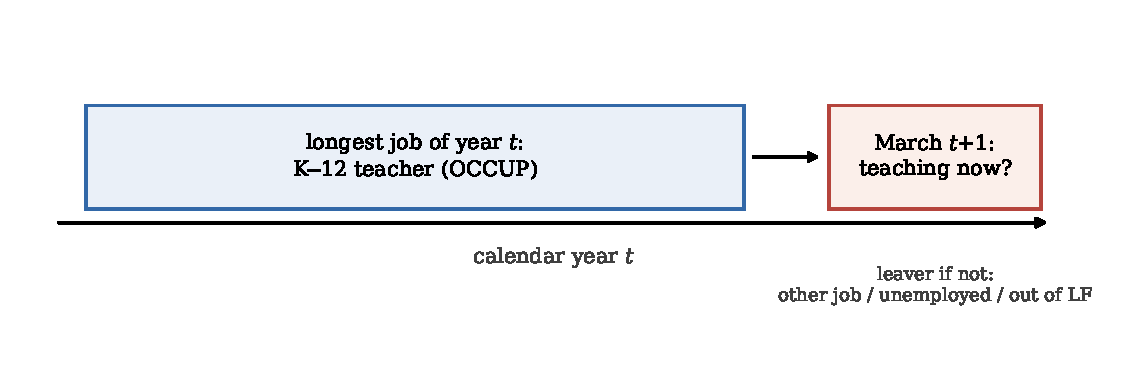
\includegraphics[width=0.9\textwidth]{figures/f1_design.pdf}
  \caption{The retrospective instrument.}
  \fignote{Each March, the ASEC records the occupation of the longest job
  held in the previous calendar year and the person's current activity.
  A teacher in year $t$ who is not teaching in March $t{+}1$ is a leaver,
  routed to another occupation, unemployment, or out of the labor force.}
\end{figure}

The data are the public-use person files of the CPS Annual Social and
Economic Supplement (ASEC) for survey years 2006--2025, downloaded from
the Census Bureau: CSV files from 2019 onward, fixed-width files parsed
against the published data dictionaries for 2011--2018, and, for
2006--2010, extracted with byte positions recovered empirically and
validated against the person identifiers of the March basic monthly
files (Appendix A describes the method). Survey year $t{+}1$ measures
attrition for calendar year $t$; the supplements cover calendar
2005--2024. The main analytical window is 2015--2024, with 2010--2014
and Harris and Adams's 1992--2001 as standing comparisons; the 2005--2009
files support the rate series only.

A person is a \textbf{teacher} in year $t$ if the occupation of her
longest job that year is K--12 classroom teaching: preschool and
kindergarten, elementary and middle school, secondary school, special
education, or teachers not elsewhere classified (census codes 2300--2330
plus 2340 under the 2002/2010 classifications and 2360 under the 2018
one; the core codes are identical across all three). Postsecondary
teachers and teaching assistants are excluded, and the main sample is
restricted to college graduates, both following
\textcolor{citeblue}{Harris and Adams (2007)}. She is a \textbf{leaver}
if in the following March she is no longer teaching, with the route read
from the labor-force recode: employed in another occupation, unemployed,
or out of the labor force. Employment status must come from the
labor-force status variable rather than the occupation field, because
the unemployed report their last job's occupation---ignoring this counts
displaced teachers as stayers. The measure captures leavers only;
teachers who change school or district remain teachers here, so these
rates sit below ``total turnover'' figures that add movers
(\textcolor{citeblue}{Ingersoll, 2001; Tan et al., 2024} report 16
percent total turnover of which roughly half is moving). Own children,
including births, are attached to each adult through the household
parent and spouse pointers. All statistics use supplement weights.

\section*{3. Who teaches}

\begin{figure}[t]
  \centering
  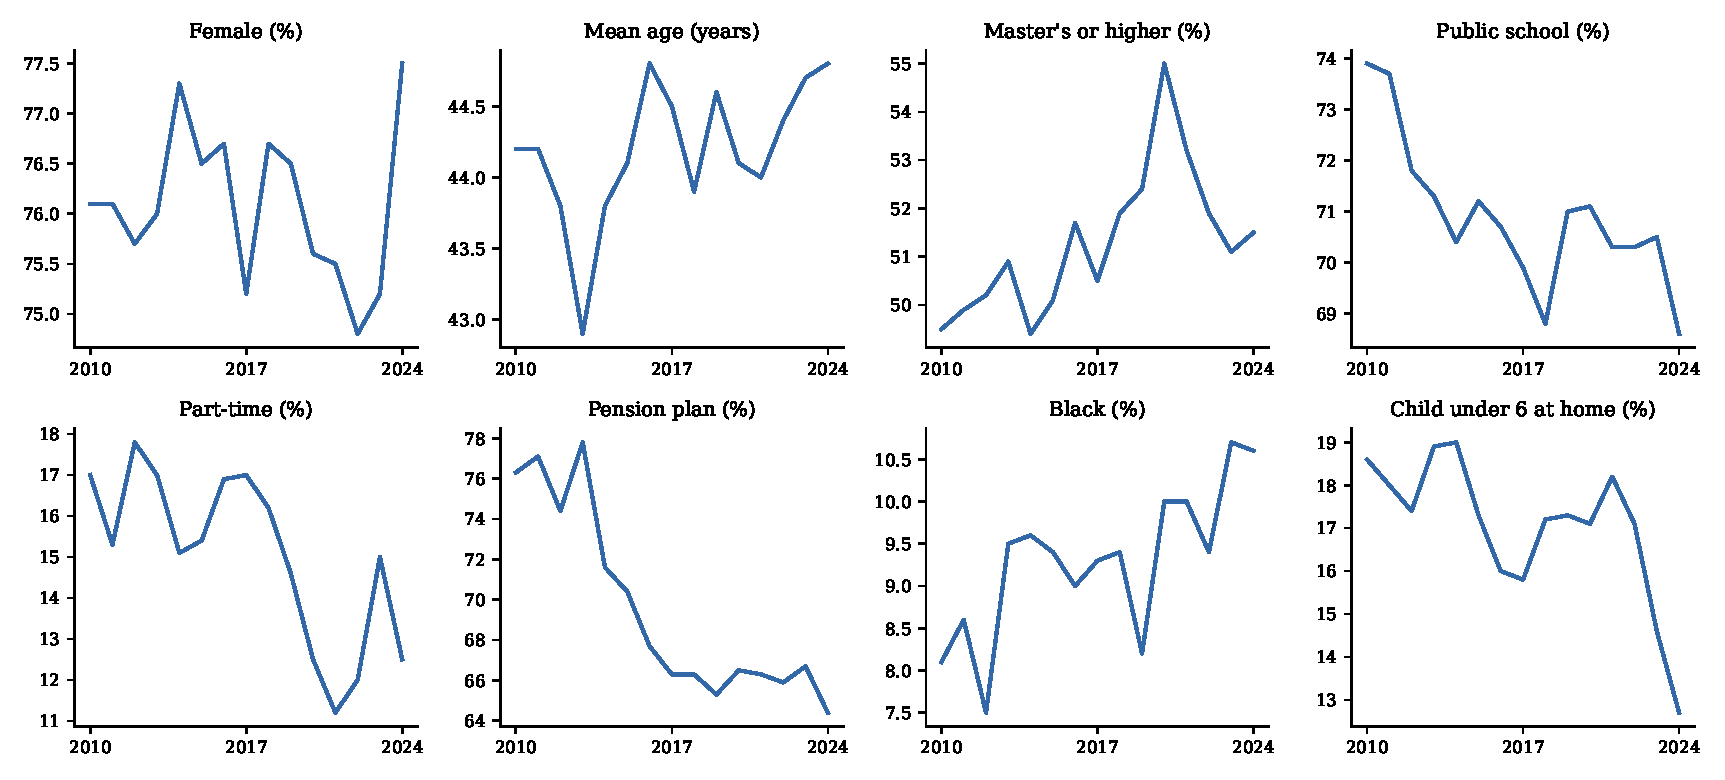
\includegraphics[width=\textwidth]{figures/f2_workforce.pdf}
  \caption{The changing profile of the teaching workforce.}
  \fignote{College-graduate K--12 teachers (longest job of the calendar
  year), ASEC 2011--2025 = calendar 2010--2024, weighted. The 2013 point
  uses the reduced five-eighths 2014 file.}
\end{figure}

The workforce against which attrition plays out has been drifting in
quiet but consistent directions. Teaching remains three-quarters female
and increasingly credentialed---the share with a master's degree or more
hovers above half---while the public-sector share has slipped and
part-time teaching has become slightly more common. Pension coverage,
teaching's signature amenity, remains near seventy percent but is
eroding at the margin. The workforce is not aging on average, a
composition effect worth keeping in mind below: high attrition at
retirement ages continuously removes the old, while entry replenishes
the young.

\section*{4. How many leave}

\begin{figure}[t]
  \centering
  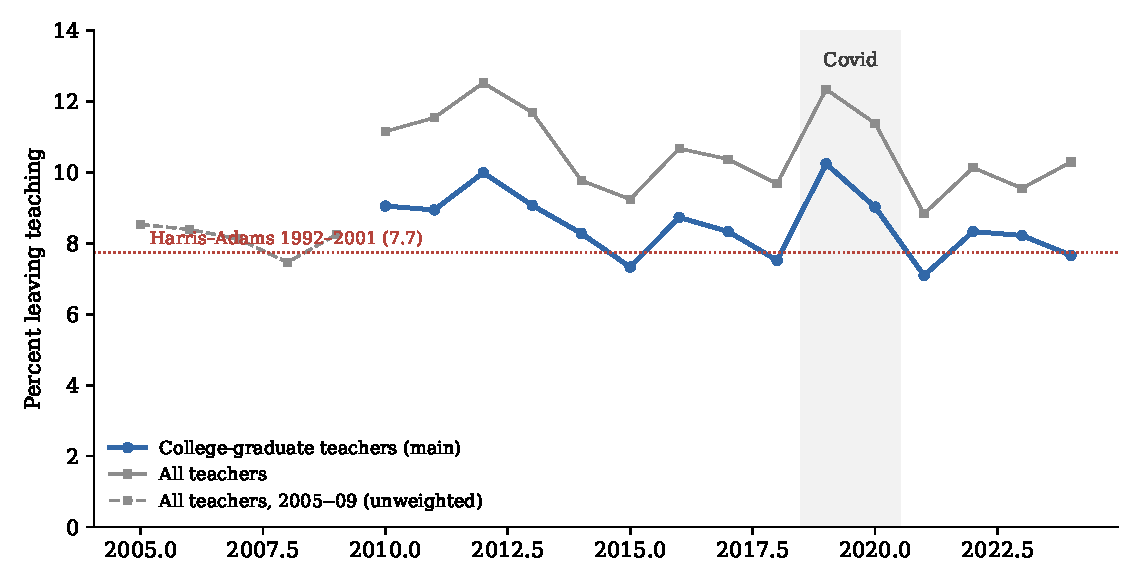
\includegraphics[width=0.92\textwidth]{figures/f3_evolution.pdf}
  \caption{Attrition by year, against a thirty-year anchor.}
  \fignote{Share of teachers (longest job of the calendar year) not
  teaching the following March. Solid blue: college graduates (main
  definition). Gray: all teachers regardless of degree. Dashed segment:
  2005--2009, unweighted counts from the minimal early extraction. The
  dotted line marks Harris and Adams's (2007) 7.73 percent for
  1992--2001 under the identical design.}
\end{figure}

Pooled over 2015--2024, \textbf{8.25 percent} of college-graduate
teachers leave the profession per year. The series wears its history
lightly: 8--9 percent in the early 2010s, 7.3--8.7 in the late 2010s, a
spike to \textbf{10.2 percent} for calendar 2019---measured in the March
2020 interviews, the first weeks of Covid---9.0 for calendar 2020, and
full reversion by 2021 (7.1), holding through 2024 (7.7). Against
Harris and Adams's 7.7 percent for 1992--2001, the conclusion is stark:
\emph{three decades of alarm about accelerating teacher flight are not
visible in the only long series measured with a constant instrument.}
The pandemic registered as a two-year disturbance, exactly as
\textcolor{citeblue}{Aldeman and Yi (2025)} conclude, and as the NCES
data ultimately showed (8.4 percent of 2020--21 teachers left before
the next school year). Within the average, the familiar structure:
public-school teachers leave at 6.8 percent, private-school teachers at
11.6---the same two-to-one ratio as in the TFS administrative
benchmarks---and men slightly exceed women (9.1 versus 8.0).

\section*{5. Where they go}

\begin{figure}[t]
  \centering
  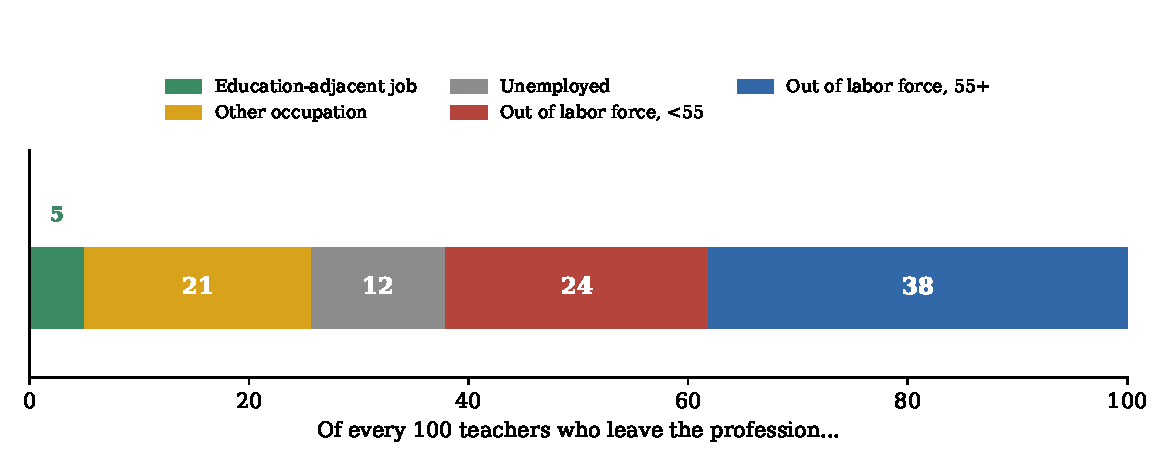
\includegraphics[width=0.96\textwidth]{figures/f4_flow100.pdf}
  \caption{Of every 100 leavers.}
  \fignote{Destinations in the March following the last teaching year,
  college-graduate teachers pooled 2015--2024, weighted.
  Education-adjacent: employed in occupations 2200--2555 (postsecondary,
  tutors, assistants, administrators, librarians).}
\end{figure}

The single most policy-relevant fact in this paper is the destination
split. Of every 100 leavers, \textbf{62 are not employed at all} a year
later: 38 have left the labor force at ages 55 and above---the
retirement channel---and 24 have left it younger, the margin where
family (Section 6) lives. Twelve are unemployed. Only \textbf{26 hold
another job}, and five of those remain in education-adjacent work:
postsecondary teaching, tutoring, school administration, teaching
assistance. The occupational destinations of the remaining switchers are
managerial and administrative far more often than technical, echoing in
survey data what \textcolor{citeblue}{Brummet et al.\ (2025)} find in
tax records. The popular narrative of attrition---teachers poached by
higher-paying industries---describes at most a fifth of actual exits.

\begin{figure}[t]
  \centering
  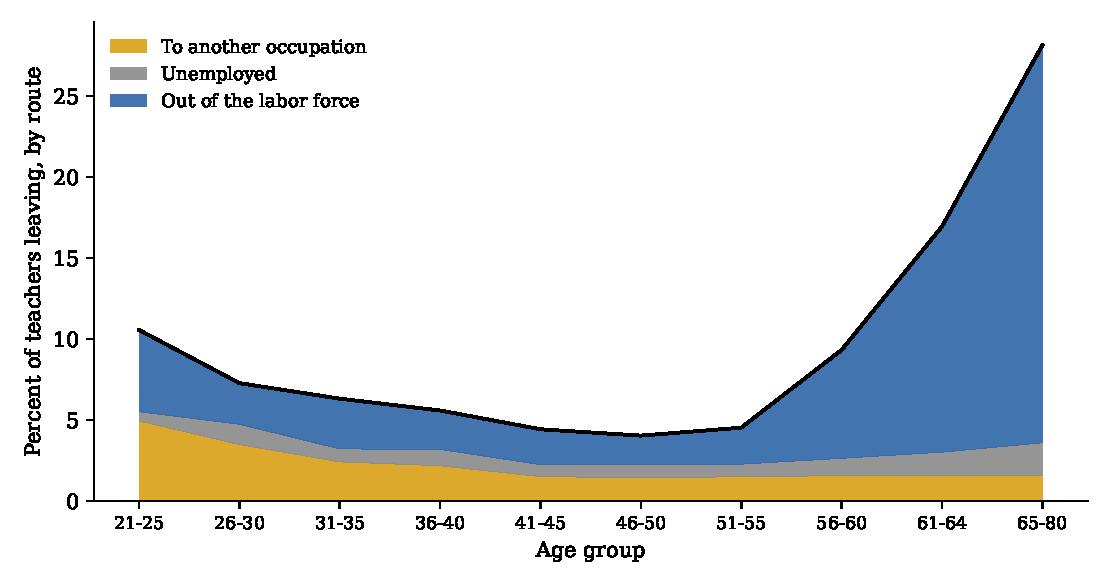
\includegraphics[width=0.9\textwidth]{figures/f5_routes_age.pdf}
  \caption{Exit routes over the lifecycle.}
  \fignote{Share of teachers leaving by each route, by age group, pooled
  2015--2024. The black line is total attrition; shaded areas stack the
  three routes.}
\end{figure}

The routes are organized by age with almost mechanical clarity.
Job-switching is a young teacher's exit: it peaks in the twenties and
declines monotonically. Labor-force exit is the mirror image, modest
through mid-career and exploding after 55; by ages 61--64 attrition is
17 percent, three quarters of it out of employment altogether. The
trough in one's forties---total attrition near 4 percent---identifies
the tenured core of the profession. This U-shape, documented for the
1990s by \textcolor{citeblue}{Grissmer and Kirby (1997)} and visible in
Harris and Adams's data, survives intact in the modern decades.

\begin{figure}[t]
  \centering
  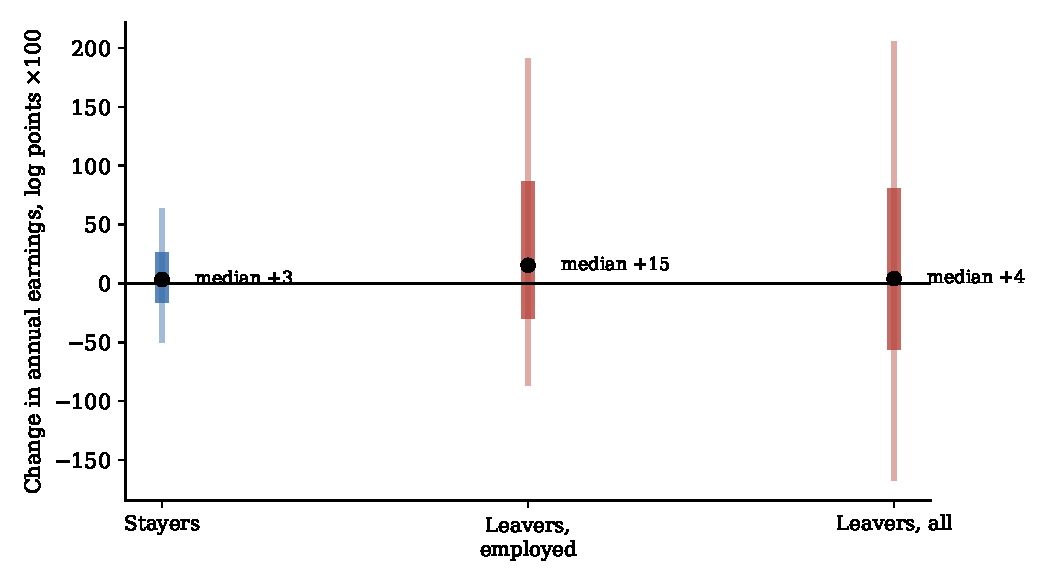
\includegraphics[width=0.84\textwidth]{figures/f6_earnings.pdf}
  \caption{The earnings gamble of leaving.}
  \fignote{Change in annual wage and salary earnings, log points
  $\times$100, from the last teaching year to the following calendar
  year, for teachers linked across consecutive March supplements by
  person identifier (validated on sex and age progression), surveys
  2011--2025. Thick bars: interquartile range; thin bars: 10th--90th
  percentiles; dots: medians. Among all leavers, 47 percent report zero
  earnings in the following year (excluded from the log-change
  distribution).}
\end{figure}

Linking the same person across consecutive Marches prices the move. For
stayers, the earnings distribution does what salary schedules promise:
a median gain of 3 log points inside a tight band. For leavers who hold
a job, the median gain is larger---15 log points---but the band
explodes: the 75th percentile gains 81 log points while the 10th
percentile \emph{loses} 85. And this is the distribution conditional on
earning anything: \textbf{47 percent of all leavers report zero
earnings} in the year after leaving. Leaving teaching for work is a
gamble that pays for the median mover and costs heavily in the tails;
leaving teaching at all is, for nearly half of leavers, a transition
into no earnings whatsoever---retirement, caregiving, or a gap year the
CPS cannot distinguish further. The ``earnings penalty of staying'' that
motivates much salary policy is nowhere visible in these transitions.

\section*{6. Who leaves, and why}

\begin{table}[t]
  \centering
  \caption{Teachers who stay versus teachers who leave.}
  \begin{tabular}{lccc}
\toprule
 & Stayers & Leavers & Difference \\
\midrule
Age, years & 43.9 & 50.1 & 6.2 \\
Female & 76.2\% & 73.4\% & -2.8\% \\
Black & 9.5\% & 10.8\% & 1.3\% \\
Married & 67.1\% & 63.7\% & -3.3\% \\
Separated or divorced & 10.2\% & 11.7\% & 1.5\% \\
Master's degree or higher & 52.4\% & 45.8\% & -6.6\% \\
Public school & 71.3\% & 58.0\% & -13.3\% \\
Enrolled in a pension plan & 68.0\% & 51.2\% & -16.8\% \\
Part-time ($<$35 h/week) & 11.9\% & 41.4\% & 29.5\% \\
Worked full year (50+ weeks) & 75.6\% & 31.3\% & -44.3\% \\
Weekly earnings (\$) & 1177.4 & 1075.0 & -102.4 \\
\bottomrule
\end{tabular}

  \fignote{Weighted means, college-graduate teachers pooled 2015--2024,
  measured in the teaching year. Earnings are annual wage and salary
  divided by weeks worked.}
\end{table}

The leaver, photographed during her last teaching year, differs from
the stayer mainly in her contract, not her demography. She is six years
older on average (the retirement tail), somewhat less likely to be in a
public school and to hold a pension, and dramatically less attached:
41 percent of leavers taught part-time (against 12 percent of stayers)
and only 31 percent worked a full 50-week year (against 76). Earnings
while teaching were about nine percent lower. Race, marriage, and
degrees move the comparison by a few points at most.

\begin{figure}[t]
  \centering
  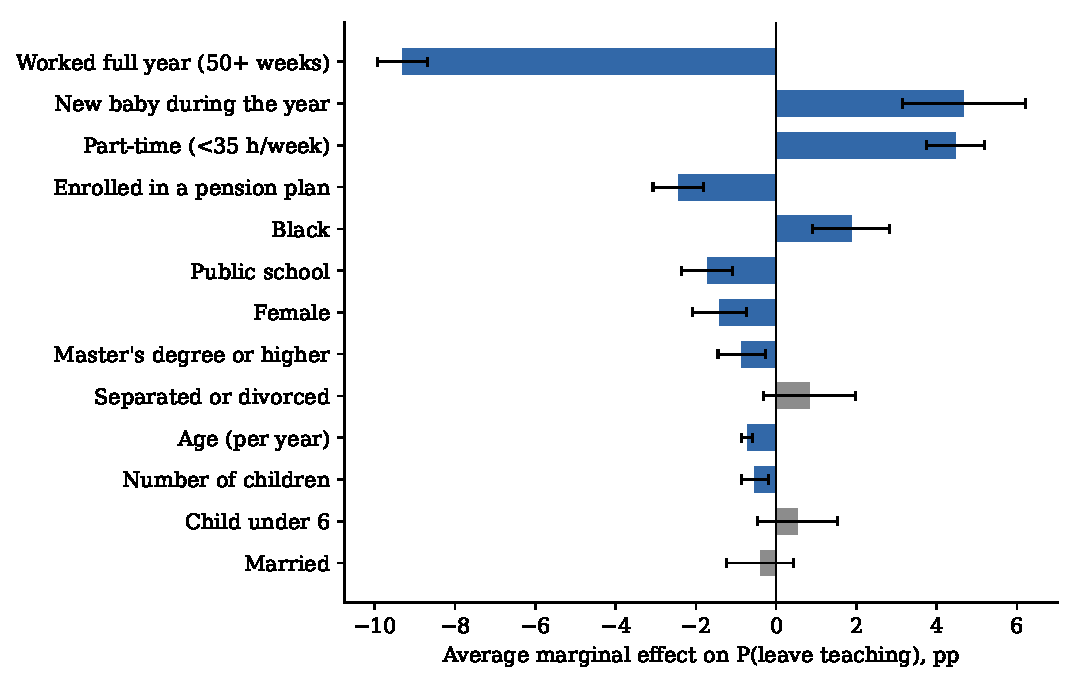
\includegraphics[width=0.92\textwidth]{figures/f7_ame.pdf}
  \caption{What predicts leaving.}
  \fignote{Average marginal effects from a probit of leaving on
  characteristics of the teaching year, with survey-year fixed effects;
  college-graduate teachers pooled 2015--2024. Whiskers: 95 percent
  confidence intervals; gray: not significant at 5 percent. Age enters
  quadratically; its profile is in Figure 5.}
\end{figure}

Multivariately, the ranking is unambiguous. Full-year work is worth
$-$9.3 percentage points of exit risk, part-time $+$4.5, pension
enrollment $-$2.4, public school $-$1.7: the attachment variables and
the deferred-compensation lock, in that order, dwarf everything
demographic. The pension coefficient echoes, at modern magnitudes, the
job-lock Harris and Adams estimated for the 1990s, and it remains two
to three times larger for teachers than for any comparison profession
(Appendix B)---the fingerprint of a profession whose exits are
choreographed by retirement systems rather than by outside offers.

The exception to ``demographics don't matter'' is the family. A birth
during the year raises a female teacher's probability of leaving by
\textbf{5.9 percentage points} (Figure 9), conditional on age,
education, marriage, and other children---an effect on the order of the
entire baseline attrition rate. The same specification estimated on
women in comparison professions yields $+$2.6 points for nurses,
$+$3.5 for accountants, $+$2.4 for lawyers, $+$2.2 for social workers:
positive everywhere, as one expects around childbirth, but \emph{two to
three times larger in teaching}. Whatever combination of parental-leave
provision, schedule rigidity during the school year, and household
specialization produces this gap, teaching loses new mothers at a rate
its semi-professional peers do not, and no amount of aggregate-level
reassurance about ``normal'' attrition addresses it.

\begin{figure}[t]
  \centering
  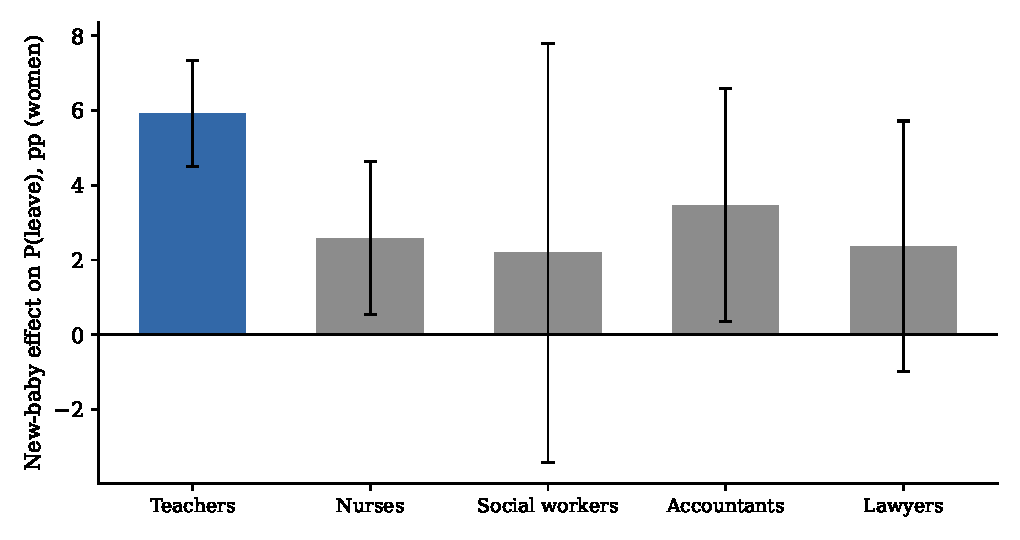
\includegraphics[width=0.8\textwidth]{figures/f9_newbaby.pdf}
  \caption{A new baby and the probability that a woman leaves her
  profession.}
  \fignote{Average marginal effect of a child under one in the
  household, from profession-specific probits on women (age quadratic,
  marriage, advanced degree, other children controls), pooled
  2010--2024. Whiskers: 95 percent confidence intervals.}
\end{figure}

\begin{table}[t]
  \centering
  \caption{The top-risk decile.}
  \begin{tabular}{lcc}
\toprule
 & Top-risk decile & All teachers \\
\midrule
\textbf{Actual leaver rate \%} & \textbf{33.0} & \textbf{8.2} \\
\midrule
Age & 54.4 & 44.4 \\
Female \% & 74.4 & 76.0 \\
Part-time \% & 75.0 & 14.3 \\
Full-year \% & 4.3 & 71.9 \\
Pension \% & 35.6 & 66.6 \\
Public \% & 45.2 & 70.2 \\
\bottomrule
\end{tabular}

  \fignote{Teachers in the top decile of predicted exit probability from
  the probit of Figure 7, versus all teachers. The model's risk
  concentrates in part-year, part-time, uncovered contracts; its
  realized attrition validates the ranking.}
\end{table}

\section*{7. Teaching among the professions}

\begin{figure}[t]
  \centering
  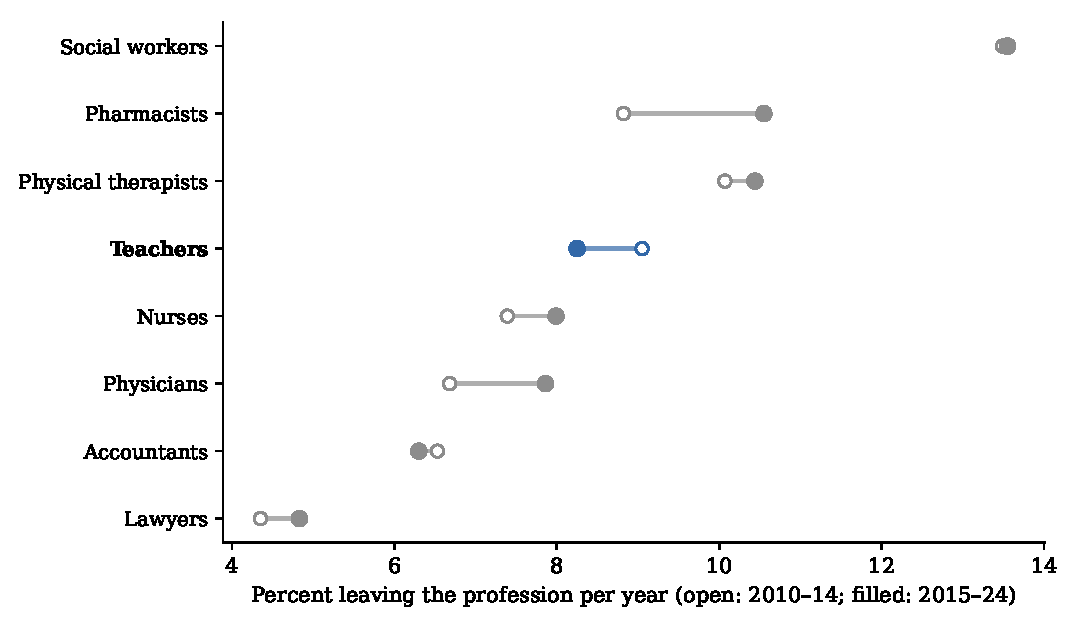
\includegraphics[width=0.9\textwidth]{figures/f8_professions.pdf}
  \caption{Leaving the profession, eight professions, two periods.}
  \fignote{Annual profession-leaving rates under the identical
  instrument, college graduates: open circles 2010--2014, filled
  2015--2024. Profession defined by the longest job of the calendar
  year; leaving includes unemployment and labor-force exit.}
\end{figure}

Is 8 percent a lot? Measured with the same ruler, teachers leave
teaching at almost exactly the rate registered nurses leave nursing
(8.0), below physical therapists (10.4) and pharmacists (10.6), five
points below social workers (13.6), and above accountants (6.3) and
lawyers (4.8). The ordering is essentially Harris and Adams's, a
generation later; the two periods shown differ by less than a point for
most professions. Teaching's true distinctions are compositional: a
larger share of its attrition exits the labor force (62 percent, versus
44 for nurses and 21 for social workers), its pension lock is stronger,
and its family margin is larger. Teaching does not have an attrition
problem relative to its peers; it has a \emph{retirement system} and a
\emph{motherhood penalty} that shape when and how its attrition
happens.

\section*{8. What it means for policy}

Three lessons follow from the anatomy rather than the level. First, the
aggregate rate is the wrong target: it has been flat for thirty years,
sits at the nurse benchmark, and its pandemic excursion self-corrected.
Retention policy motivated by a supposed exodus is aiming at a ghost.
Second, the actionable margins are visible and specific: part-year and
part-time attachments carry many times the exit risk of any demographic
group; pension coverage retains; and the family channel---a five-point
exit effect of a birth, unmatched in comparable professions---points
directly at leave policy and within-year schedule flexibility as the
binding constraints on retaining young mothers. Third, the destination
evidence disciplines the rhetoric of competition: schools are not
losing teachers to industry in any volume; they are losing them to
retirement, to family, and to nothing at all. For the minority who do
move, the move is a high-variance gamble, not a raise---which suggests
the outside option constrains teacher retention far less than the
inside conditions do.

\section*{References}

\begin{itemize}[leftmargin=1.2em,itemsep=2pt,label={}]
\item Aldeman, C., and S. Yi (2025). ``Are Teachers Abandoning Their
Profession in Large Numbers?'' \textit{Education Next}.
\item Brummet, Q., E. Penner, N. Pharris-Ciurej, and S. Porter (2025).
``After School: An Examination of the Career Paths and Earnings of Former
Teachers.'' \textit{Educational Evaluation and Policy Analysis}.
\item Carver-Thomas, D., and L. Darling-Hammond (2017). \textit{Teacher
Turnover: Why It Matters and What We Can Do About It}. Learning Policy
Institute.
\item Chetty, R., J. Friedman, and J. Rockoff (2014). ``Measuring the
Impacts of Teachers II: Teacher Value-Added and Student Outcomes in
Adulthood.'' \textit{American Economic Review} 104(9).
\item Grissmer, D., and S. Kirby (1997). ``Teacher Turnover and Teacher
Quality.'' \textit{Teachers College Record} 99(1).
\item Harris, D., and S. Adams (2007). ``Understanding the Level and
Causes of Teacher Turnover: A Comparison with Other Professions.''
\textit{Economics of Education Review} 26(3).
\item Henke, R., and L. Zahn (2001). \textit{Attrition of New Teachers
Among Recent College Graduates}. NCES.
\item Ingersoll, R. (2001). ``Teacher Turnover and Teacher Shortages: An
Organizational Analysis.'' \textit{American Educational Research
Journal} 38(3).
\item Madrian, B., and L.~J. Lefgren (2000). ``An Approach to
Longitudinally Matching Current Population Survey Respondents.''
\textit{Journal of Economic and Social Measurement} 26(1).
\item Nguyen, T., L. Pham, M. Crouch, and M. Springer (2020). ``The
Correlates of Teacher Turnover: An Updated and Expanded Meta-analysis.''
\textit{Educational Research Review} 31.
\item Podgursky, M. (2003). ``Fringe Benefits.'' \textit{Education Next}
3(3).
\item Rivkin, S., E. Hanushek, and J. Kain (2005). ``Teachers, Schools,
and Academic Achievement.'' \textit{Econometrica} 73(2).
\item Ronfeldt, M., S. Loeb, and J. Wyckoff (2013). ``How Teacher
Turnover Harms Student Achievement.'' \textit{American Educational
Research Journal} 50(1).
\item Stinebrickner, T. (2002). ``An Analysis of Occupational Change and
Departure from the Labor Force: Evidence of the Reasons that Teachers
Leave.'' \textit{Journal of Human Resources} 37(1).
\item Tan, T., W. Wei, D. Carver-Thomas, and E. García (2024).
\textit{Teacher Turnover in the United States: Who Moves, Who Leaves,
and Why}. Learning Policy Institute.
\end{itemize}

\clearpage
\section*{Appendix A. Validating the instrument person by person}

Because the CPS interviews each address in four consecutive months, rests
it for eight, and interviews it again in the same four calendar months a
year later, individuals can be linked across interviews
(\textcolor{citeblue}{Madrian and Lefgren, 2000}) and teacher attrition
can, in principle, be measured prospectively. We built this panel from
the raw monthly files---twenty entry cohorts, 2005--2024---keeping the
unambiguous teachers (employed in K--12 teaching in all four initial
interviews) and defining a panel-leaver as one who teaches in none of the
four follow-up interviews. For the subsample whose initial window
includes March, the same person also answered the following year's ASEC
retrospective questions, and the two instruments can be cross-tabulated
individual by individual. The same person identifiers link the
supplement to the monthly files; for supplement years whose fixed-width
layouts predate the published dictionaries, byte positions were recovered
by scanning for the offset at which the 22-character person identifier
reproduces the March monthly identifiers---a join that cannot succeed by
accident---and validated on occupation agreement in the interview week.

\begin{table}[h]
  \centering
  \caption{Panel classification versus March retrospective, twenty
  cohorts.}
  \begin{tabular}{lcccc}
\toprule
 & \multicolumn{3}{c}{March retrospective classification} & \\
\cmidrule(lr){2-4}
Linked-panel classification & Not a teacher & Stayed & Left & Total \\
\midrule
Stayer (teaches all 4 post months) & 198 & 7,911 & 67 & 8,176 \\
Leaver (teaches in none) & 1,018 & 10 & 257 & 1,285 \\
\midrule
Total & 1,216 & 7,921 & 324 & 9,461 \\
\bottomrule
\end{tabular}

  \fignote{Teachers stable across all four initial monthly interviews,
  observed in all four follow-ups, window including March, linked to the
  following ASEC (n = 9{,}461). ``Not a teacher'': the retrospective
  codes the longest job of the base year outside K--12 teaching.}
\end{table}

Wherever the two instruments agree the person was a base-year teacher,
they almost never disagree about what happened next: \textbf{99.1
percent} agreement, 77 true conflicts in 9,461 cases, stable at 98--100
percent in every cohort. The entire distance between the panel's
apparent attrition (13.6 percent among these stable teachers) and the
retrospective's (3.9 percent) lives in the 13 percent of panel-teachers
whom the retrospective does not count as teachers at all---and their
longest jobs are teaching assistant, other-instructor, education
administrator, postsecondary teacher, childcare: the education-adjacent
boundary, plus reference-week noise (summer non-employment, temporary
absences) that a single-week snapshot cannot avoid. The panel measures
leaving the \emph{classroom this week}; the retrospective measures
leaving the \emph{profession this year}. For this paper's questions the
second is the estimand, and the audit shows it is measured consistently
---which is also why the raw point-in-time panel rates that circulate in
policy debates (15 percent and above) should not be read as profession
exit.

\section*{Appendix B. Harris and Adams (2007) on the modern decades}

\begin{table}[h]
  \centering
  \caption{Leaving the profession, by type: 1992--2001 versus 2015--2024.}
  \begin{tabular}{lcccccccc}
\toprule
 & \multicolumn{4}{c}{Harris \& Adams, 1992--2001} & \multicolumn{4}{c}{This paper, 2015--2024} \\
\cmidrule(lr){2-5}\cmidrule(lr){6-9}
 & All & Switch & Unemp. & Out LF & All & Switch & Unemp. & Out LF \\
\midrule
Teachers & 7.73 & 2.59 & 0.61 & 4.53 & 8.25 & 2.12 & 1.00 & 5.12 \\
Nurses & 6.09 & 1.68 & 0.86 & 3.54 & 7.99 & 3.66 & 0.81 & 3.53 \\
Social workers & 14.94 & 10.87 & 1.34 & 2.73 & 13.55 & 9.45 & 1.22 & 2.89 \\
Accountants & 8.01 & 4.10 & 1.55 & 2.36 & 6.30 & 1.79 & 1.18 & 3.32 \\
\bottomrule
\end{tabular}

  \fignote{Annual rates in percent, college graduates, March CPS.
  1992--2001 from Harris and Adams (2007, Tables 1--2); 2015--2024
  computed here. ``Switch'': employed in another occupation; ``Out LF'':
  out of the labor force in the survey week.}
\end{table}

Their design, applied verbatim to 2015--2024, returns their world with
minor drift: teaching within half a point of its 1990s level, still
indistinguishable from nursing once composition is controlled (the
teacher--nurse gap ranges from $+$0.3 to $-$1.8 points across control
sets), still five-plus points below social work. Teaching's labor-force
exit share---59 percent of attrition then, 62 now---and its outsized
pension coefficient ($-$3.6 percentage points, versus $-$1.1 to $-$1.6
in the comparison professions) both survive. A literature that has spent
two decades relitigating whether teacher attrition is exceptional can
treat the question as closed: it was not then, and it is not now. What
this paper adds is everything the level conceals.

\section*{Appendix C. Additional estimation output}

\begin{table}[h]
  \centering
  \caption{Annual attrition series, 2005--2024.}
  \begin{tabular}{lcccc}
\toprule
Calendar year & College graduates & All teachers & Observations & Weighted \\
\midrule
2005 & -- & 8.5\% & 4,161 & no \\
2006 & -- & 8.4\% & 4,336 & no \\
2007 & -- & 8.1\% & 4,357 & no \\
2008 & -- & 7.5\% & 4,448 & no \\
2009 & -- & 8.2\% & 4,357 & no \\
2010 & 9.1\% & 11.2\% & 4,301 & yes \\
2011 & 8.9\% & 11.5\% & 4,184 & yes \\
2012 & 10.0\% & 12.5\% & 4,192 & yes \\
2013 & 9.1\% & 11.7\% & 2,896 & yes \\
2014 & 8.3\% & 9.8\% & 4,333 & yes \\
2015 & 7.3\% & 9.2\% & 3,972 & yes \\
2016 & 8.7\% & 10.7\% & 4,045 & yes \\
2017 & 8.3\% & 10.4\% & 4,053 & yes \\
2018 & 7.5\% & 9.7\% & 3,986 & yes \\
2019 & 10.2\% & 12.3\% & 3,321 & yes \\
2020 & 9.0\% & 11.4\% & 3,232 & yes \\
2021 & 7.1\% & 8.8\% & 3,040 & yes \\
2022 & 8.3\% & 10.1\% & 3,141 & yes \\
2023 & 8.2\% & 9.6\% & 3,006 & yes \\
2024 & 7.7\% & 10.3\% & 2,918 & yes \\
\bottomrule
\end{tabular}

  \fignote{College-graduate and all-teacher definitions. The 2005--2009
  supplements support only the minimal extraction (occupation pairs);
  their rates are unweighted and shown for the trend only. The 2013 row
  uses the reduced five-eighths 2014 file.}
\end{table}

\begin{table}[h]
  \centering
  \caption{Determinants of leaving teaching: full probit.}
  \begin{tabular}{lcc}
\toprule
 & AME (pp) & SE \\
\midrule
Age (per year) & -0.72 & (0.07) \\
age2 & 0.01 & (0.00) \\
Female & -1.41 & (0.34) \\
Black & 1.87 & (0.49) \\
Married & -0.40 & (0.43) \\
Separated or divorced & 0.83 & (0.58) \\
Master's degree or higher & -0.86 & (0.30) \\
Public school & -1.72 & (0.32) \\
Enrolled in a pension plan & -2.44 & (0.32) \\
Part-time (<35 h/week) & 4.47 & (0.37) \\
Worked full year (50+ weeks) & -9.31 & (0.32) \\
Number of children & -0.53 & (0.17) \\
Child under 6 & 0.53 & (0.51) \\
New baby during the year & 4.67 & (0.78) \\
\bottomrule
\end{tabular}

  \fignote{Average marginal effects, percentage points; college-graduate
  teachers pooled 2015--2024 with survey-year fixed effects. Children
  variables from household parent and spouse pointers.}
\end{table}

\begin{table}[h]
  \centering
  \caption{Destination occupations of switchers.}
  \begin{tabular}{lc}
\toprule
Destination occupation & Share of switchers \\
\midrule
Managers, all other & 6.0\% \\
Postsecondary teachers & 4.9\% \\
Education and childcare administrators & 4.2\% \\
Lawyers & 3.7\% \\
Postsecondary teachers & 3.6\% \\
Tutors & 2.6\% \\
Teaching assistants & 2.6\% \\
Teaching assistants & 2.3\% \\
Childcare workers & 2.3\% \\
Customer service representatives & 2.1\% \\
Secretaries and administrative assistants, except legal, medical, and executive & 1.7\% \\
Retail salespersons & 1.3\% \\
\bottomrule
\end{tabular}

  \fignote{Detailed destination occupations among leavers employed at
  $t{+}1$, pooled 2015--2024; 19.5 percent of switchers remain in
  education occupations.}
\end{table}

\end{document}
